\chapter{Research Design and Methodology}
\section{Design-science strategy and what counts as evidence}

This dissertation uses an applied design-science strategy because the research object is a working
portfolio-reporting artefact for a bounded organisational problem. Design science links construction
to evaluation against stated objectives \citep{hevner2004design,peffers2007dsrm}. The method therefore
separates three kinds of evidence: implementation records show what was built, engineering tests show
which specified behaviours were exercised, and D0 shows how two workflow conditions handled labelled
fictional cases.

The student built and evaluated the artefact, which creates confirmation risk. The main controls were
fixed case labels and metrics, versioned code and fixtures, saved result files, complete failure
accounting and repeated runs \citep{pineau2021reproducibility,nist2023airmf}. These controls make
changes visible. They do not provide independent validation.

A small set of designed cases is easily mistaken for a weak substitute for a large sample. Ribeiro
and colleagues argue the opposite for behavioural testing: held-out accuracy on a single test set
overstates real capability, and a structured suite of targeted cases, each built to probe one
specified behaviour, exposes failures that aggregate scores conceal \citep{ribeiro2020checklist}.
That is the warrant for D0. Kapoor and Narayanan show how easily designed or leaky setups flatter a
system \citep{kapoor2023leakage}. Read together, the two support a diagnostic rather than estimative
reading: passing D0 shows that a targeted control is present.

Figure~\ref{fig:meth-design-science-evidence-chain} shows the evidence boundary used throughout the
study. The figure's reporting stage is labelled for RQ1--RQ2, which are the only active questions.
Manual work, participant review, live-web operation and managed-platform comparison were
removed from the active research questions because they had no authorised observations
\citep{nist2023airmf,hevner2004design}. Table~\ref{tab:meth-evidence-scope} is the single downstream
reference for that cut.

\begin{figure}[htbp]
  \centering
  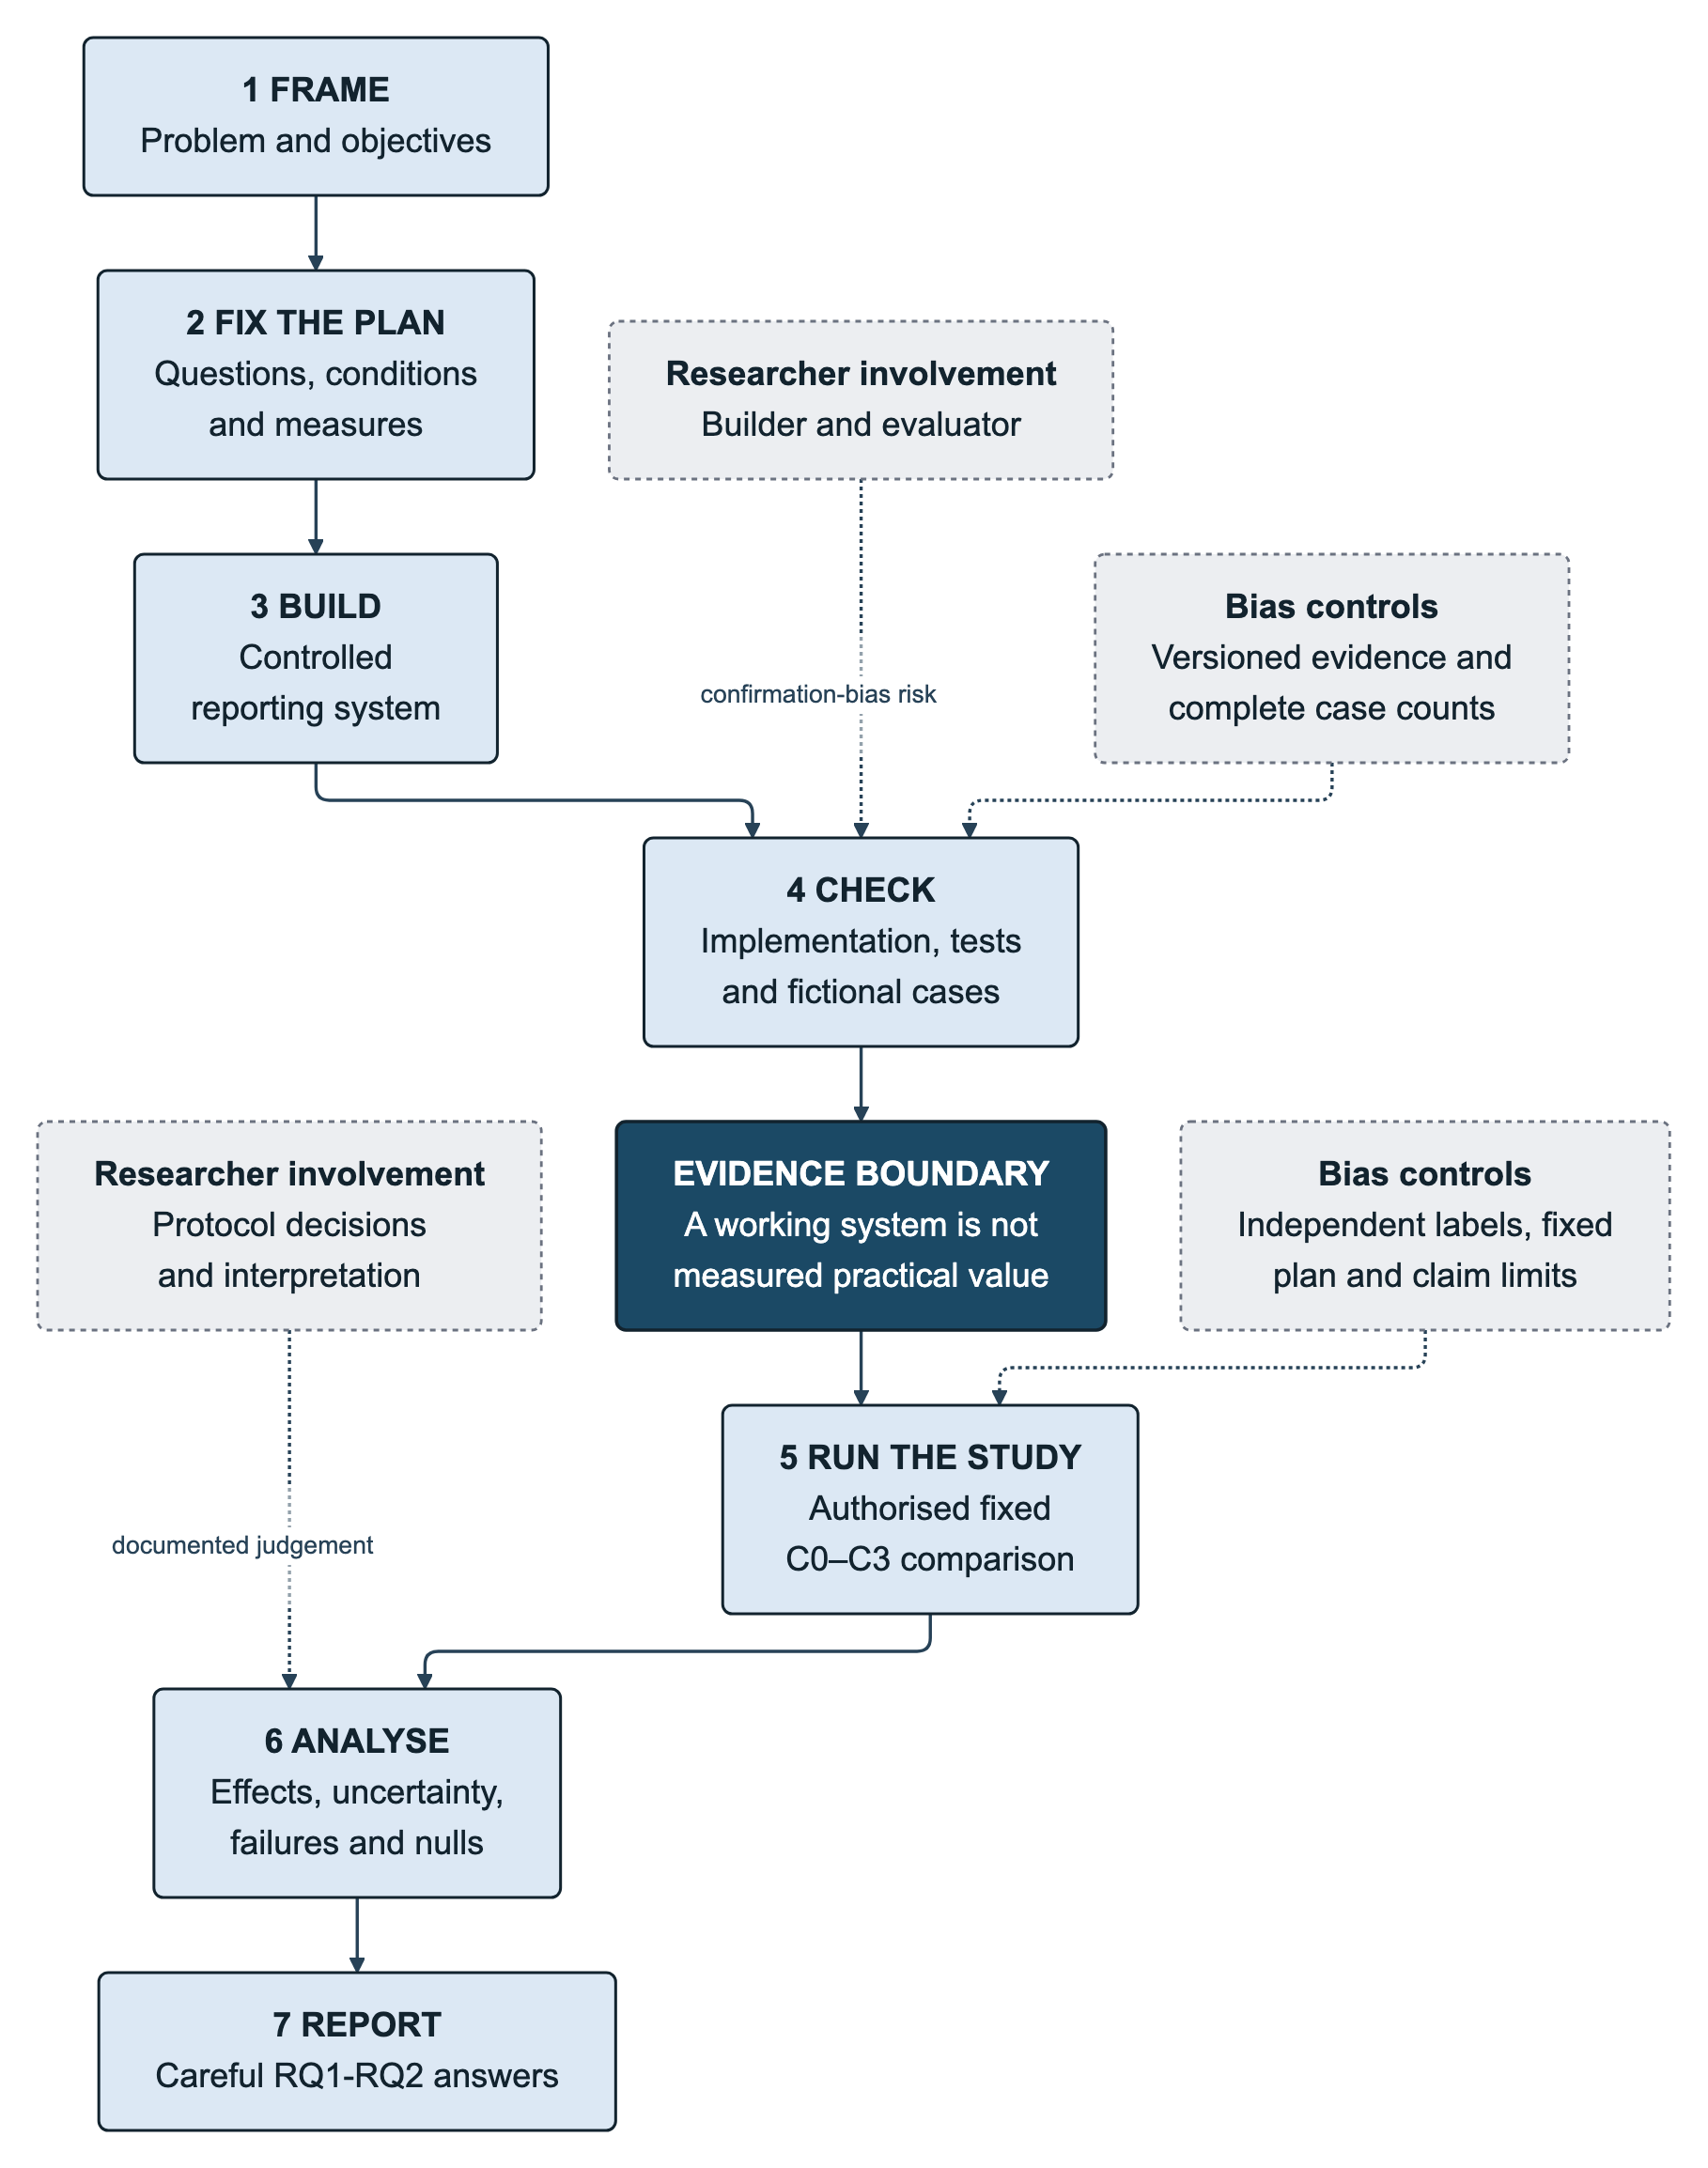
\includegraphics[width=\textwidth,height=0.82\textheight,keepaspectratio]{exhibits/meth_f1_design_science_evidence_chain.png}
  \caption{Boundary between construction, engineering checks and study results. Developed by the
  author from the cited methods literature and the project's fixed rules.}
  \label{fig:meth-design-science-evidence-chain}
\end{figure}

\section{Design decisions and rejected alternatives}

I chose fourteen cases across thirteen designed categories, with two probes in the
blank-versus-zero category, because the question is whether a specified gate fires, not what
rate it would achieve on a population of companies. A further case in the same category would
still be a designed probe. It would not become a sample. Ribeiro's checklist logic is the
reason for that shape \citep{ribeiro2020checklist,kapoor2023leakage}. The categories are
complete and sparse records, blank against observed zero, mixed types, conflicting and stale
evidence, unsupported and inaccessible sources, unclear identity, duplicate support, narrative
evidence, mixed currencies and prompt injection. A single designed probe per remaining
category is enough to ask whether the named gate fires. The blank-versus-zero pair is the
exception, because collapsing those two states is the error the catalogue exists to prevent.
That shape is still not enough to say how often a gate would fire on a portfolio, which is why
Chapter~5 reports case decisions beside the rates
\citep{ribeiro2020checklist,pineau2021reproducibility}.

I chose synthetic material because it supplies controlled labels. Bradley and colleagues show that
empty cells, zeros and table positions are easy to confuse in financial extraction, which is exactly
the distinction D0 needs to hold visible \citep{bradley2024synfintabs,gebru2021datasheets}. A real
company panel would have been preferable for transfer. It was not used here because independent
labels, a sealed freeze and authority to process restricted portfolio data were not available. That
absence is sequenced in Section~\ref{sec:sequencing-unrun}, not treated as a silent omission.

Three repeats are there to test exact repeatability of a programmed gate, not to estimate variance
in a sample. Reproducibility guidance asks for enough procedure that another person can inspect the
route to a result \citep{pineau2021reproducibility,mitchell2019modelcards}. The first repeat is
scored. The complete ordered outcome list is compared across all three. Agreement is therefore a
property of the fixture and the code, not a confidence interval.

Precision, recall and F1 are used because RQ2 is about claim admission, not about cost or speed.
Precision asks what share of emitted claims were supported. Recall asks whether required supported
claims were kept. The unsupported-claim rate uses the same emitted-claim denominator as precision.
Cost-weighted scores would have mixed a mechanism question with an efficiency question that D0
cannot answer, because both routes are local fixed rules with truncated sub-millisecond times
\citep{gao2023alce,gao2023rarr}.

C1 versus C2 is the comparison because Fu and colleagues show that extra agents are not a result
until inputs are held equal. Under matched conditions, at most one of six multi-agent systems beat
the single-agent anchor \citep{fu2026agents,guo2024multiagent}. That preprint is the warrant for
giving C1 and C2 the same cases, catalogue, candidate values and evidence, and for refusing to read
the difference as a verdict on multi-agent design. What differs is a separately recorded verification
stage that can refuse claim admission. Composition cannot override that decision
\citep{wu2024autogen,peffers2007dsrm}.

I also rejected a third D0 cell that would have pretended to be a manual baseline. Writing a
human-looking score beside the same fixture would have looked like C0 without being one. Fu and
colleagues' matched-input requirement applies to that temptation as well: a fake manual cell
would not have held effort, sources or stopping rules equal
\citep{fu2026agents,kapoor2023leakage}. The honest C0 belongs in the authorised pilot, where a
person and the workflow see the same company-periods.

The evaluand is the complete local workflow configuration: input rules, catalogue, source access,
operational roles, verification, prompts, schemas, computing environment and stop conditions.
Design-science evaluation requires comparison with stated objectives, and system reporting should
state the intended use, version and evaluation procedure
\citep{hevner2004design,mitchell2019modelcards}. The original protocol also defined C0 manual work
and C3 named review. Those conditions did not run. Their detailed condition matrix is kept as
Table~\ref{tab:meth-condition-matrix} in Appendix~\ref{app:dataset-source-freeze}, so the planned
comparison remains inspectable without presenting missing observations as evidence
\citep{pineau2021reproducibility,nist2023airmf}.

For D0, both conditions receive the same candidate value, evidence record, reporting period and
precondition. Scoring uses the fixture's expected emission and status fields. The evaluator does not
give either condition later evidence or a wider source window. This equal-input design is sufficient
for the narrow C1/C2 mechanism comparison. The visible development labels are not an independent
reference \citep{kapoor2023leakage,pineau2021reproducibility}. A real-company evaluation would
require an eligible-source list, cut-off date, independently labelled claims and recorded
adjudication, and agreement would indicate consistency rather than truth because reviewers can share
an error \citep{artstein2008agreement,gao2023alce}.

\section{What was validated and what was not}
\label{sec:evidence-scope}

Table~\ref{tab:meth-evidence-scope} classifies every downstream claim in this dissertation as
validated, built but not evaluated, or planned only. Engineering tests and D0 sit in the first
column. The public-web route, live official connectors and live company-research sit in the second.
Manual work, named review, sealed evaluation and the business pilot sit in the third
\citep{hevner2004design,pineau2021reproducibility}. Later chapters cite this table rather than
restating the cut.

\begin{table}[htbp]
  \centering
  \small
  \setlength{\tabcolsep}{3pt}
  \renewcommand{\arraystretch}{1.12}
  \begin{tabularx}{\textwidth}{@{}P{0.30\textwidth}P{0.34\textwidth}Y@{}}
    \toprule
    \textbf{Validated in this study} &
    \textbf{Built, not evaluated} &
    \textbf{Planned only} \\
    \midrule
    Local identity, missing-state, period, provenance, verification, approval and export controls.
    Paired C1/C2 D0 on fourteen labelled fictional cases, three repeats.
    286 automated tests on the 28~August~2026 snapshot.
    Offline connector replay and controlled adversarial tests with fake providers. &
    Live public-web discovery, capture and extraction.
    Direct live Companies House and UKRI retrieval (held at gate G2).
    External-model extraction on real companies (only synthetic smoke runs exist).
    Live company-research against an open website. &
    Manual baseline C0.
    Named-review condition C3.
    D1 independent labels and sealed D2.
    Managed-platform comparison.
    Accessibility and independent security assessment.
    Authorised business pilot. \\
    \bottomrule
  \end{tabularx}
  \caption{Evidence scope for this dissertation}
  \label{tab:meth-evidence-scope}
  \vspace{3pt}
  \parbox{\textwidth}{\scriptsize
    \textit{Source note:} Author classification of the executed snapshot, the repository and the
    unrun protocols. Later chapters cite this table rather than restating the boundary.}
\end{table}


The three columns are mutually exclusive for any given claim. A passing engineering test cannot be
read as a live-source result, and an unrun protocol cannot be read as a negative finding
\citep{hevner2004design,pineau2021reproducibility}. The left-hand column is the only column
Chapter~5 may treat as a result. The middle column is why Chapter~4 can describe a public-web
funnel without Chapter~5 reporting a live-web accuracy: the code exists, the specified control
fired on fake providers, and no authorised live endpoint was contacted. The right-hand column is
why interviews, a manual baseline and a usability study are absent from the results rather than
reported as zeros \citep{kapoor2023leakage,fu2026agents}. Reading down the table is therefore a
reading rule for the rest of the report. Later chapters point back to it instead of restating
that cut. The planned-only column is also why this chapter does not invent a substitute
observation. An interview summary, an expert rating or a usability score that was never
collected cannot be inferred from the existence of a review screen
\citep{amershi2019guidelines,bucinca2021forcing}. The table is the place those absences are
named once.

\section{D0 fixture}

D0 contains fourteen visible, labelled fictional cases. The fixture and its evaluation record are
checksum-pinned. Loading checks the schema version, data classification, source version, file
checksum and test-only namespace. Case and evidence identifiers sit in a benchmark namespace that
the operational collector rejects. The complete case ledger is
Table~\ref{tab:appendix-d0-case-ledger} in Appendix~\ref{app:supplementary-evaluation}
\citep{gebru2021datasheets,pineau2021reproducibility}.

Error-detection and error-injection studies give the same warrant as Ribeiro. Detectors on
ReaLMistake run at very low recall compared with humans, whose agreement reached an F1 of 95.7
\citep{kamoi2024realmistake,ribeiro2020checklist}. On SummExecEdit the best joint detect-and-explain
score was 0.49, and 60 inconsistent summaries were missed by every model tested
\citep{thorat2024summexecedit,kamoi2024realmistake}. D0 is therefore written as labelled refusals of
claim admission, including the fixture outcome held, which this dissertation uses as a refusal or
non-admission label rather than as a human hold.

D0 is a development fixture. The rules and cases were written together, so the result establishes
only whether the programmed gate behaves as designed on these cases. A future pilot must create
independent labels before a sealed final set is opened \citep{kapoor2023leakage,pineau2021reproducibility}.

Error analysis uses the expected verification states and records false emission, false withholding,
conflict, stale evidence, inaccessible evidence, identity hold and untrusted content separately.
Negative and unavailable outcomes remain in the record. Any later study should pair the same
company-periods, report exclusions before rates and use uncertainty at the company or report level,
not treat repeated fields as independent observations
\citep{kapoor2023leakage,pineau2021reproducibility}.

\section{Measures and denominators}

The primary D0 measures are supported-claim precision, recall, F1, unsupported-claim rate,
source-record completeness and exact repeat consistency. Table~\ref{tab:meth-primary-denominators}
states the denominators used in Chapter~5. Contradiction accuracy has two applicable cases and is
read as a small case result, not a stable rate. Duration values below one millisecond were truncated
to zero. Model cost is zero because D0 uses fixed local rules. Measures without D0 labels remain
null, not zero \citep{gao2023alce,nikiforova2020quality}.

\begin{table}[htbp]
  \centering
  \small
  \setlength{\tabcolsep}{3pt}
  \renewcommand{\arraystretch}{1.12}
  \begin{tabularx}{\textwidth}{@{}P{0.28\textwidth}P{0.32\textwidth}Y@{}}
    \toprule
    \textbf{Measure} & \textbf{Numerator / denominator} & \textbf{Why it is used} \\
    \midrule
    Supported-claim precision & Supported emitted claims / all emitted claims & Does refusal raise the share of admitted claims that are supported? \\
    Recall & Correctly emitted required claims / all required claims & Does refusal drop claims that should have been said? \\
    Unsupported-claim rate & Unsupported emitted claims / all emitted claims & The complement of precision on the same emitted set. \\
    Source-record completeness & Complete source records / emitted claims & Completeness of the record, not discovery of new sources. \\
    Exact repeat consistency & Identical ordered outcomes across three repeats & Repeatability of the programmed gate. \\
    \bottomrule
  \end{tabularx}
  \caption{Primary D0 denominators}
  \label{tab:meth-primary-denominators}
  \vspace{3pt}
  \parbox{\textwidth}{\scriptsize
    \textit{Source note:} Compact view of the metric matrix in
    Appendix~\ref{app:supplementary-evaluation}. Cost, time and reviewer measures have no D0 labels
    and remain null.}
\end{table}


The complete metric matrix in Appendix~\ref{app:supplementary-evaluation} also defines prospective
human time, edit, usability and cost measures. Those fields are pilot metrics, not results of this
study \citep{nist2023airmf,pineau2021reproducibility}. No inferential test is reported, because
D0 is not a sample \citep{ribeiro2020checklist,kapoor2023leakage}.
The evaluator reports counts before rates and keeps all fourteen paired cases in both conditions.
Individual cases explain why an aggregate changed. Schema and normalisation accuracy are also
reported because both conditions share earlier processing, so a difference there would not be a
verifier effect \citep{gao2023alce,pineau2021reproducibility}. Contradiction accuracy uses two
applicable cases. Reporting it as 0.000 versus 1.000 is honest about those two cases and
misleading if read as a stable detector rate. Duration and model cost stay in the record as
truncated zeros so that a later reader can see they were collected and were uninformative,
rather than quietly dropped \citep{gebru2021datasheets,nikiforova2020quality}.

\section{Scope decisions: no interviews, no manual baseline}
\label{sec:sequencing-unrun}

Interviews, expert ratings and a stakeholder usability study were not run. They would have required
authorised participants, a frozen protocol and a recorded coding frame. Those observations do not
exist, so they are not inferred from the interface
\citep{amershi2019guidelines,bucinca2021forcing}. Promised-but-unrun interview or rating work is
therefore absent from Chapter~5. It is not reported as a weak result or as a zero score.

A manual baseline was postponed for the same sequencing reason, not as an apology. Fu and colleagues
show that a comparison that does not hold inputs equal cannot attribute a gain to extra machinery
\citep{fu2026agents,peffers2007dsrm}. A C0 cell that used different sources, a different cut-off or
a different completion rule would not isolate the verifier. I did not run interviews because they
would have answered a different question: how operators talk about reporting, not whether a
programmed refusal changes claim admission under matched inputs. A usability study of the review
screen would likewise measure preference and effort, not support
\citep{amershi2019guidelines,bucinca2021forcing}. The matched manual comparison therefore belongs
in the authorised pilot in Section~\ref{sec:business-pilot}, where the same company-periods,
source window and stopping rule can be frozen before anyone sees the outcomes
\citep{kapoor2023leakage,pineau2021reproducibility}.

\section{Ethics, data classification, reproducibility}
\label{sec:ethics}

Every input is classified as restricted, internal, public or synthetic. Restricted material remains
local. Public availability does not itself authorise every use
\citep{gebru2021datasheets,cddo2023genai,nist2023airmf}. D0 uses only fictional data and no external
source or model call. Local copies are checksum-linked, written once where required, kept out of Git
and privately permissioned. Personal contact details are removed before an accepted public page is
stored.

The optional external route sends only approved public or synthetic company-level material. It
requires open collection and model gates, reviewed identity, a named reviewer, an approved route and
a runtime key. Requests use \texttt{store=False}, strict schemas and fixed limits. Bounded
synthetic smoke runs were executed on that optional route. The run manifests are not in this
tree. The current code pins \texttt{gpt-5.6-luna}. Those runs are connectivity evidence, not a
result. No restricted, internal or real-company material was sent. OpenAI separates saved
application state from abuse-monitoring retention, and \texttt{store=False} is not Zero Data
Retention \citep{openai2026datacontrols,cddo2023genai}.

The evaluation record retains the Git revision and dirty-state warning, platform and dependency
versions, migration version, fixture and protocol checksums, test commands, result files, failures
and output hashes. Collection stops when authority is unclear, a credential is exposed, unexpected
personal data appears, source terms would be breached, restricted data would reach an unapproved
service, or a sealed evaluation set is compromised
\citep{pineau2021reproducibility,nist2023airmf}. The report links company events to evidence. It does
not advise buying or selling, rank companies, or profile individuals
\citep{fca2024promotions,cddo2023genai}. These controls define the research boundary. They do not
imply ethics approval for the future pilot.

Public pages may contain hidden instructions, misleading identities or malformed content. The route
treats downloaded text as data, limits model tools, rejects instruction-like passages and demands
exact support before it accepts a claim. The tests cover chosen risks; the controls cannot spot every
hostile form \citep{greshake2023indirect,autio2024genai}. Collection checks the protocol, embedded
credentials, ports, network addresses, redirects, robots rules, content type, elapsed time and
decompressed size, and connects to a verified public address while still checking the certificate
hostname. Controlled tests covering internal-service access, address switching, redirects, content
type and size all passed. Each test confirms that one specified input was refused
\citep{autio2024genai,nist2023airmf}. Budgets, bounded retries, cancellation, task fingerprints,
checksums and staged export together limit runaway cost, stale completion, altered files and partial
writes. A forced stop can still leave work that needs deliberate recovery
\citep{pineau2021reproducibility,nist2023airmf}.

Work with real restricted data or with participants stays held until an approved data-management and
ethics plan names who controls the data and who owns purpose, access, retention, deletion and incident
response. No retention period has been invented in the meantime. What the prototype demonstrates is a
local purpose limit, which is a design property rather than a data-protection judgement
\citep{nist2023airmf,cddo2023genai}. The research concerns companies, not individuals. Captured
contact details are removed; director, employee, investor or journalist profiles, inferred sensitive
traits and reputation scores are excluded. A named public statement may support a relevant company
claim but cannot become a judgement about that person. Human approval cannot expand these limits
\citep{cddo2023genai,nist2023airmf}.
